% Nội dung ElasticNet và LightGBM, chia 4 section theo cấu trúc chương của báo cáo:
%   Section 1 -> Chương 2 (Cơ sở lý thuyết)
%   Section 2 -> Chương 3 (Phương pháp nghiên cứu)
%   Section 3 -> Chương 4 (Kết quả và thảo luận)
%   Section 4 -> Chương 5 (Kết luận và hướng phát triển)
% Có thể chuyển từng section sang đúng chương khi tổng hợp; các nhãn \ref giữa các section vẫn dùng được.
%
% Tài liệu tham khảo dùng trong phần này (cần có trong danh sách tham khảo chung):
% [Zou & Hastie, 2005] H. Zou, T. Hastie, "Regularization and variable selection via the elastic net",
%     Journal of the Royal Statistical Society: Series B, 67(2), 301--320, 2005.
% [Friedman, 2001] J. H. Friedman, "Greedy function approximation: a gradient boosting machine",
%     The Annals of Statistics, 29(5), 1189--1232, 2001.
% [Chen & Guestrin, 2016] T. Chen, C. Guestrin, "XGBoost: a scalable tree boosting system",
%     Proceedings of the 22nd ACM SIGKDD International Conference on Knowledge Discovery and Data Mining, 785--794, 2016.
% [Ke et al., 2017] G. Ke et al., "LightGBM: a highly efficient gradient boosting decision tree",
%     Advances in Neural Information Processing Systems 30, 2017.
% [Pedregosa et al., 2011] F. Pedregosa et al., "Scikit-learn: machine learning in Python",
%     Journal of Machine Learning Research, 12, 2825--2830, 2011.
% [De Cock, 2011] D. De Cock, "Ames, Iowa: alternative to the Boston housing data as an end of semester
%     regression project", Journal of Statistics Education, 19(3), 2011.

% ======================================================================
\section{Cơ sở lý thuyết: ElasticNet, LightGBM và thang đo}
\label{sec:theory-b}

\subsection{ElasticNet}
\label{subsec:elasticnet}

ElasticNet (Zou và Hastie, 2005) tối thiểu hàm mục tiêu kết hợp phạt $\ell_1$ và $\ell_2$:
\begin{equation}
\min_{w} \frac{1}{2n}\,\|y-Xw\|_2^2
+ \alpha\,\rho\,\|w\|_1
+ \frac{\alpha\,(1-\rho)}{2}\,\|w\|_2^2,
\qquad \rho=\texttt{l1\_ratio}\in[0,1].
\end{equation}
Với $\rho=0$ thu được Ridge, với $\rho=1$ thu được Lasso (tự chọn đặc trưng); giá trị giữa dùng $\ell_1$ để
sparse và một phần $\ell_2$ để ổn định khi các biến tương quan. Vì cả hai phạt cộng trực tiếp theo độ lớn hệ số,
mô hình \textbf{nhạy với thang đo} đầu vào, do đó biến số được chuẩn hóa bằng \texttt{StandardScaler}
(median impute kèm missing indicator) và biến danh mục được one-hot. Sau \texttt{FeatureBuilder} (86 cột),
không gian đầu vào là 334 cột số.

\subsection{Gradient boosting và LightGBM}
\label{subsec:lightgbm}

Gradient boosting (Friedman, 2001) xây mô hình cộng $\hat y_i=\sum_{k=1}^{K}\eta\,f_k(x_i)$, trong đó mỗi cây
hồi quy $f_k$ được thêm tuần tự để giảm hàm mất mát (ở đây là sai số bình phương trên $\log(1+\text{price})$),
$\eta=\texttt{learning\_rate}$ là hệ số co. Theo khai triển của Chen và Guestrin (2016), mỗi cây được chọn bằng
xấp xỉ bậc hai của mất mát theo gradient $g_i$ và hessian $h_i$ của dự đoán hiện tại, có phạt $\ell_2$ trên giá
trị lá:
\begin{equation}
\min_{f}\ \sum_i\Big[g_i f(x_i)+\tfrac12 h_i f(x_i)^2\Big]+\tfrac12\lambda\sum_{j=1}^{T} w_j^2 ,
\qquad \lambda=\texttt{reg\_lambda},
\end{equation}
với $T$ lá và giá trị lá $w_j$. LightGBM (Ke và cộng sự, 2017) tìm ngưỡng tách bằng histogram và mọc cây theo
lá (leaf-wise) giới hạn bởi \texttt{num\_leaves}, nên nhanh trên nhiều cột. Mô hình \textbf{không scale, không
impute}: numeric NaN được giữ nguyên và cây tự học hướng đi mặc định cho missing; biến danh mục ở dạng pandas
\texttt{category} với từ điển học chỉ trên phần huấn luyện, cấp chưa gặp rơi vào nhánh NaN, nên không cần one-hot
và giữ đúng 86 cột. Cây không phụ thuộc thang đo nên không cần chuẩn hóa.

Ý nghĩa các siêu tham số được tìm kiếm: \texttt{n\_estimators} là số cây $K$; \texttt{learning\_rate} là $\eta$
(nhỏ hơn cần nhiều cây hơn nhưng ít overfit hơn); \texttt{num\_leaves} là số lá tối đa $T$ của mỗi cây (độ phức
tạp); \texttt{min\_child\_samples} là số mẫu tối thiểu trong một lá (giá trị nhỏ cho phép lá bắt cả nhiễu);
\texttt{subsample} là tỉ lệ dòng được lấy mẫu cho mỗi cây (bagging); \texttt{colsample\_bytree} là tỉ lệ cột được
dùng cho mỗi cây; \texttt{reg\_lambda} là $\lambda$ trong công thức trên.

\subsection{Thang đo đánh giá}

Với giá thật $y_i$, dự đoán $\hat y_i$ và $n$ mẫu:
$\text{MAE}=\frac1n\sum_i|y_i-\hat y_i|$,
$\text{RMSE}=\sqrt{\frac1n\sum_i(y_i-\hat y_i)^2}$,
$R^2=1-\sum_i(y_i-\hat y_i)^2\big/\sum_i(y_i-\bar y)^2$ và
$\text{MAPE}=\frac{100}{n}\sum_i|y_i-\hat y_i|/y_i$.
MAE được dùng để chọn cấu hình vì có đơn vị USD dễ diễn giải và ít bị chi phối bởi vài giao dịch cực đoan hơn
RMSE; giá nhà lệch phải nên RMSE và $R^2$ nhạy với ngoại lai.

% ======================================================================
\section{Phương pháp huấn luyện, tuning và đánh giá}
\label{sec:method-b}

Hai mô hình được tinh chỉnh siêu tham số bằng \texttt{GridSearchCV} (ElasticNet) và \texttt{RandomizedSearchCV}
(LightGBM) của scikit-learn (Pedregosa và cộng sự, 2011) trên 5-fold CV chung của nhóm, chọn theo MAE tính trên
USD. Cả hai huấn luyện trên $\log(1+\text{price})$ và đưa dự đoán về USD trước khi tính mọi metric. Mô hình chốt
được đánh giá trên 586 mẫu test sau khi cấu hình đã chốt, và so với mốc tham chiếu là dự đoán hằng số bằng median
giá dev.

\subsection{Tuning ElasticNet}

\begin{itemize}
  \item \textbf{Giai đoạn 1 (grid thô):} $\alpha\in$ \texttt{logspace}$(-5,0,19)$
    $\times$ $\rho\in\{0;0{,}1;0{,}3;0{,}5;0{,}7;0{,}9;0{,}95;1\}$, 152 cấu hình $\times$ 5 fold.
  \item \textbf{Giai đoạn 2 (tinh chỉnh):} 13 giá trị $\alpha$ quanh điểm tối ưu, $\rho\in\{0{,}9;0{,}95;0{,}99\}$.
  \item \textbf{Đối chứng target identity:} $\alpha\in$ \texttt{logspace}$(-1,4,15)$ (90 cấu hình), thang $\alpha$
    dịch lên vì nhãn USD cần phạt lớn hơn nhãn log để có cùng mức regularization.
\end{itemize}
Hai đầu $\rho=0$ và $\rho=1$ chỉ làm mốc tham chiếu (Ridge/Lasso-like); cấu hình chốt thuộc miền hỗn hợp
$0<\rho<1$. Mô hình chốt hội tụ trong \texttt{max\_iter=10000} ở cả 5 fold.

\subsection{Tuning LightGBM}

\texttt{RandomizedSearchCV} lấy 40 trên 5.184 cấu hình, mỗi cấu hình 5 fold (200 lần fit), chấm bằng MAE USD:
\texttt{n\_estimators} $\in\{300;500;700;1000\}$, \texttt{learning\_rate} $\in\{0{,}03;0{,}05;0{,}1\}$,
\texttt{num\_leaves} $\in\{15;31;63\}$, \texttt{min\_child\_samples} $\in\{5;10;20;40\}$,
\texttt{colsample\_bytree} $\in\{0{,}6;0{,}8;1\}$, \texttt{subsample} $\in\{0{,}7;0{,}9;1\}$,
\texttt{reg\_lambda} $\in\{0;1;5;10\}$. Target identity được đối chứng tại đúng cấu trúc chốt; target log1p được
giữ nếu identity không tốt hơn quá 1\%.

\subsection{Phân tích ngoại lai và độ nhạy}

Vì kết quả bị chi phối bởi một số giao dịch cực đoan, so sánh hai mô hình được lặp lại sau khi loại các nhà trên
4.000~sqft. Tiêu chí này theo khuyến nghị của tài liệu bộ dữ liệu (De Cock, 2011), chỉ dùng diện tích, không dùng
giá hay residual, phù hợp chính sách ``không lọc holdout theo target''. Độ bất định được ước lượng bằng bootstrap
ghép cặp (5.000 lần) trên 586 nhà test, và bằng so sánh theo dòng trên dự đoán out-of-fold gộp của 5-fold CV. Đây
là phân tích mô tả thực hiện sau khi đã có kết quả test, không dùng để chọn lại mô hình.

% ======================================================================
\section{Kết quả và thảo luận}
\label{sec:results-b}

\subsection{Kết quả tuning và CV}

\textbf{ElasticNet.} Cấu hình thắng CV: $\alpha=5{,}41\times10^{-5}$, $\rho=0{,}99$, target $\log(1+\text{price})$
(CV MAE 14.660). Target identity cho 16.107 (kém 9\%; lưới chỉ 90 cấu hình và không gồm $\rho=0{,}99$ nên mức
chênh chỉ mang tính tham khảo). Hai mốc $\rho=0$ và $\rho=1$ cho 15.167 và 14.680. MAE tốt nhất theo $\rho$ giảm
từ 15.167 ở $\rho=0$ xuống 14.666 ở $\rho=0{,}95$ và gần như đi ngang khi $\rho\geq0{,}5$ (chênh khoảng 0,7\%);
chênh lệch giữa $\rho=0{,}99$ và Lasso thuần chỉ 20~USD (0,14\%), nhỏ hơn nhiều so với std giữa các fold, nên không
thể khẳng định thành phần $\ell_2$ giúp ích. Đường CV MAE theo $\alpha$ (hình~\ref{fig:enet-alpha}) có cực tiểu
rộng: thay $\alpha$ trong khoảng 16 lần quanh điểm tối ưu chỉ làm MAE đổi dưới 2\%.

\textbf{LightGBM.} Cấu hình thắng: \texttt{n\_estimators}=700, \texttt{learning\_rate}=0,03, \texttt{num\_leaves}=15,
\texttt{min\_child\_samples}=5, \texttt{colsample\_bytree}=0,8, \texttt{subsample}=0,7, \texttt{reg\_lambda}=5 (CV MAE
13.600). Target identity tại cấu trúc này cho 13.858, kém log1p 1,9\%. Cần đọc kết quả thận trọng: ba siêu tham số
(\texttt{learning\_rate}, \texttt{num\_leaves}, \texttt{min\_child\_samples}) rơi đúng giá trị nhỏ nhất của lưới nên
điểm tối ưu có thể nằm ngoài lưới, và ba cấu hình đầu bảng có CV MAE 13.600, 13.624, 13.634, chênh nhau dưới 0,3\%
(nhỏ hơn nhiều so với std giữa fold, khoảng 1.000) nên thứ hạng giữa chúng không đáng tin.

\begin{figure}[H]\centering
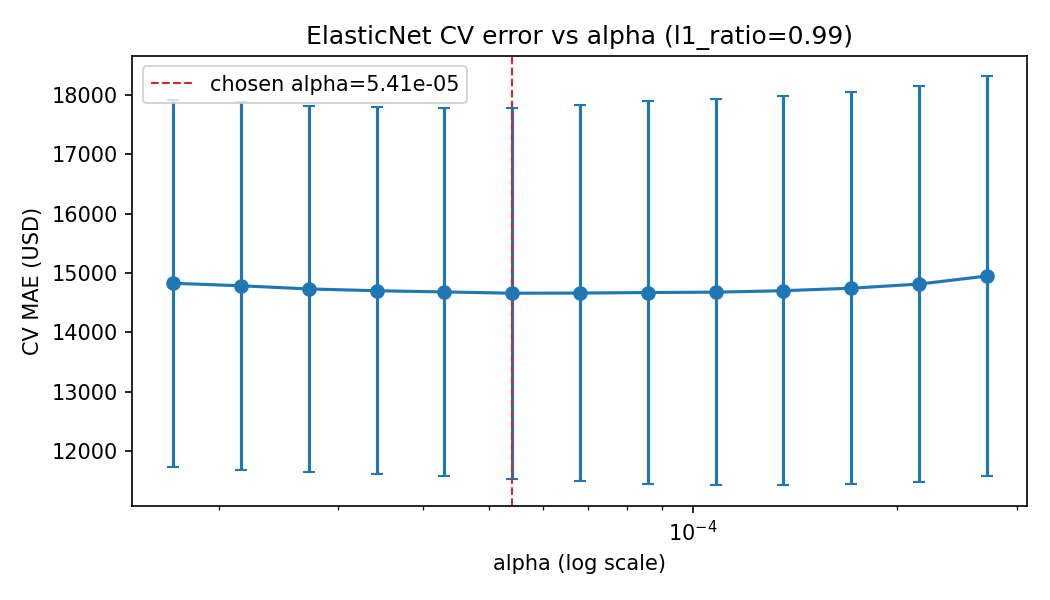
\includegraphics[width=.7\linewidth]{figures/enet_alpha_curve.png}
\caption{CV MAE của ElasticNet theo $\alpha$ tại $\rho$ chốt; thanh lỗi là std giữa các fold (ddof=0 do
\texttt{GridSearchCV} tính, các bảng dùng ddof=1).}
\label{fig:enet-alpha}
\end{figure}

\begin{table}[H]
\centering\small
\begin{tabular}{lrrrrrr}
\toprule
 & \multicolumn{2}{c}{MAE} & \multicolumn{2}{c}{RMSE} & \multicolumn{2}{c}{$R^2$} \\
\cmidrule(lr){2-3}\cmidrule(lr){4-5}\cmidrule(lr){6-7}
Fold & ElasticNet & LightGBM & ElasticNet & LightGBM & ElasticNet & LightGBM \\
\midrule
1 & 12.553 & 12.554 & 18.078 & 20.221 & 0,945 & 0,931 \\
2 & 13.673 & 13.430 & 20.288 & 21.376 & 0,923 & 0,915 \\
3 & 20.855 & 14.952 & 102.036 & 31.212 & $-$0,707 & 0,840 \\
4 & 12.810 & 12.759 & 17.353 & 18.198 & 0,939 & 0,932 \\
5 & 13.409 & 14.306 & 19.434 & 27.827 & 0,949 & 0,896 \\
\midrule
mean & 14.660 & 13.600 & 35.438 & 23.767 & 0,610 & 0,903 \\
std & 3.492 & 1.019 & 37.247 & 5.505 & 0,736 & 0,038 \\
\bottomrule
\end{tabular}
\caption{CV 5-fold của hai mô hình chốt (USD); std theo mẫu (ddof=1). MAPE trung bình của CV được nêu ở
bảng~\ref{tab:compare-b}.}
\label{tab:cv-b}
\end{table}

\textbf{Overfitting.} Sau khi refit trên toàn dev, MAE ``trong mẫu'' của LightGBM là 6.382 so với CV MAE 13.600
(gap $\times$2,1), lớn hơn nhiều so với ElasticNet (11.691 so với 14.660, gap $\times$1,25). Đây là đặc trưng của
boosting trên tập nhỏ. Test MAE của LightGBM (13.060) nằm trong dao động của CV MAE ($\pm$1.019), nên không thấy
dấu hiệu overfit vào bước chọn mô hình; việc test thấp hơn một chút cũng có thể do mô hình cuối được huấn luyện
trên nhiều dòng hơn (2.344 so với khoảng 1.875 dòng mỗi fold).

\subsection{Hệ số của ElasticNet và tầm quan trọng đặc trưng của LightGBM}

ElasticNet giữ 233/334 hệ số khác 0. Vì target là log-price, hệ số $\beta$ trên biến số đã chuẩn hóa diễn giải
gần đúng là hiệu ứng giá $(e^{\beta}-1)$ cho mỗi 1 độ lệch chuẩn; $\beta$ của cột one-hot (không chuẩn hóa) là hiệu
ứng của việc nhà \emph{có} cấp đó so với \emph{không có}.

\begin{table}[H]
\centering\small
\begin{tabular}{lrrl}
\toprule
Đặc trưng & $\beta$ & $e^{\beta}-1$ & Số nhà trong dev \\
\midrule
roof\_matl\_ClyTile & $-$2,267 & $-$89,7\% & \textbf{1} \\
misc\_feature\_Elev & $-$1,700 & $-$81,7\% & \textbf{1} \\
functional\_Sal & $-$1,283 & $-$72,3\% & \textbf{1} \\
neighborhood\_GrnHill & $+$0,453 & $+$57,2\% & \textbf{2} \\
mas\_vnr\_type\_CBlock & $-$0,203 & $-$18,4\% & \textbf{1} \\
gr\_liv\_area & $+$0,165 & $+$18,0\% & (biến liên tục) \\
overall\_qual & $+$0,121 & $+$12,8\% & (biến liên tục) \\
quality\_x\_living\_area & $-$0,123 & $-$11,5\% & (biến liên tục) \\
\bottomrule
\end{tabular}
\caption{Một số hệ số có $|\beta|$ lớn (không liệt kê hết, ví dụ ms\_zoning\_C và heating\_Grav cũng lớn). Năm hệ số
đầu nằm trên các cấp one-hot chỉ có 1--2 quan sát.}
\end{table}

Năm hệ số lớn nhất đều rơi vào cấp one-hot rất hiếm: ``mái ngói đất nung rẻ đi 90\%'' hay ``nhà có thang máy giảm
82\%'' không phải quy luật thị trường mà là hệ số khớp cho đúng 1--2 nhà huấn luyện. Với các biến ``thật'',
gr\_liv\_area và overall\_qual có dấu hợp lý. Hệ số âm của quality\_x\_living\_area không nên đọc riêng lẻ vì biến
này tương quan rất mạnh với hai biến thành phần trên tập dev (Pearson 0,92 với gr\_liv\_area và 0,81 với
overall\_qual); chỉ hiệu ứng gộp của bộ ba mới có nghĩa.

Theo gain, \texttt{quality\_x\_living\_area} chiếm 46,5\% tổng gain của LightGBM, tiếp theo là overall\_qual
(11,1\%), living\_plus\_total\_basement\_sf (8,0\%) và neighborhood (7,8\%) (hình~\ref{fig:lgbm-imp}). Năm đặc trưng
do nhóm tạo trong top 20 chiếm 57,5\% tổng gain, nghĩa là mô hình dựa nhiều vào chúng; do chưa có ablation bỏ các
đặc trưng engineered nên chưa thể kết luận chúng làm giảm sai số. Gain là thước đo tương quan, không phải nhân
quả, và thiên về biến liên tục có nhiều ngưỡng tách. Trên test, MAE theo neighborhood cao nhất ở Crawfor (33.019,
14 nhà), NridgHt (31.301, 45 nhà) và StoneBr (28.027, 15 nhà), thấp nhất ở SWISU (6.924); theo năm bán MAE dao động
11.977--15.525 (cao nhất năm 2009), nhưng vì \texttt{yr\_sold} là đầu vào nên một phần hiệu ứng năm có thể là ghi
nhớ chu kỳ thị trường 2006--2010.

\begin{figure}[H]\centering
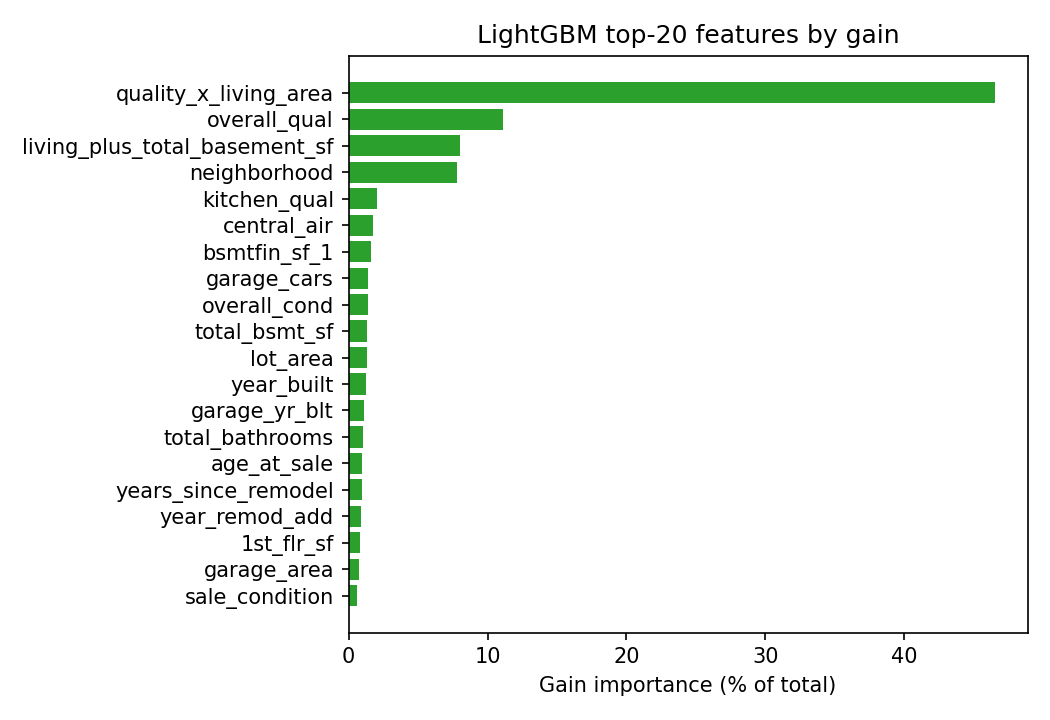
\includegraphics[width=.7\linewidth]{figures/lgbm_importance.png}
\caption{Top-20 đặc trưng theo gain của LightGBM chốt.}
\label{fig:lgbm-imp}
\end{figure}

\subsection{So sánh ElasticNet và LightGBM}

\begin{table}[H]
\centering
\begin{tabular}{lrrrr}
\toprule
 & \multicolumn{2}{c}{Test (586 nhà)} & \multicolumn{2}{c}{CV 5-fold (mean)} \\
\cmidrule(lr){2-3}\cmidrule(lr){4-5}
Metric (USD) & ElasticNet & LightGBM & ElasticNet & LightGBM \\
\midrule
MAE & 14.267 & \textbf{13.060} & 14.660 & \textbf{13.600} \\
RMSE & 31.954 & \textbf{21.149} & 35.438 & \textbf{23.767} \\
$R^2$ & 0,873 & \textbf{0,944} & 0,610 & \textbf{0,903} \\
MAPE (\%) & 7,78 & \textbf{6,90} & 9,08 & \textbf{8,24} \\
\bottomrule
\end{tabular}
\caption{Hai mô hình trên cùng holdout và cùng giao thức CV. LightGBM có số tốt hơn ở mọi metric. $R^2$ CV của
ElasticNet bị kéo xuống bởi fold 3 (trung vị các fold: 0,939). Mốc tham chiếu (dự đoán hằng số bằng median giá
dev) trên test: MAE 63.838, RMSE 94.323, $R^2=-0{,}110$, MAPE 33,0\%.}
\label{tab:compare-b}
\end{table}

\begin{figure}[H]\centering
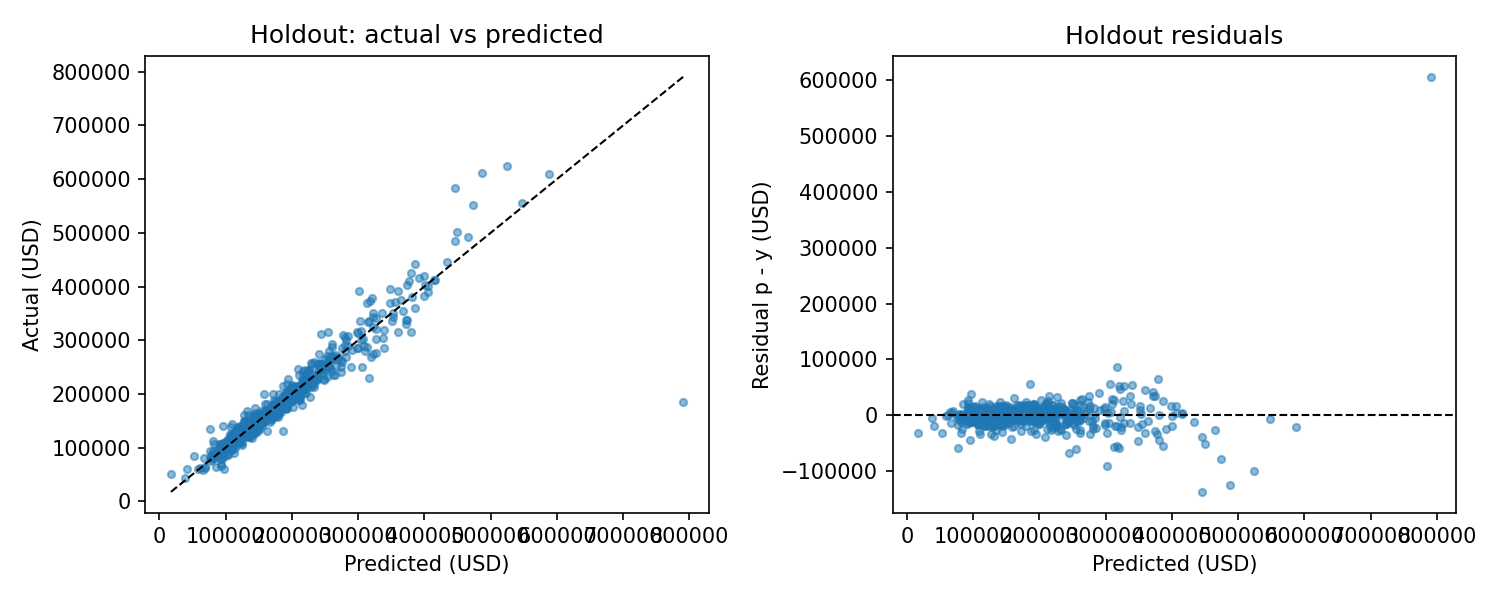
\includegraphics[width=.8\linewidth]{figures/enet_residuals.png}\\[2pt]
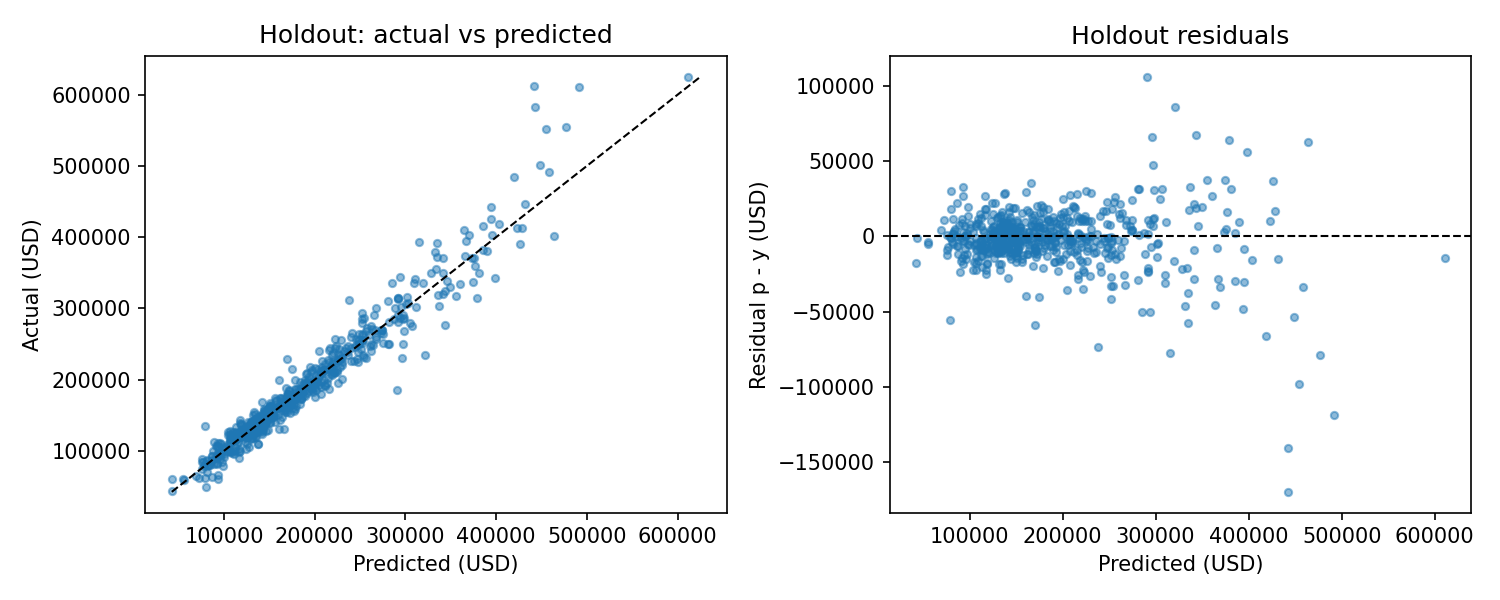
\includegraphics[width=.8\linewidth]{figures/lgbm_residuals.png}
\caption{Thực tế so với dự đoán và residual trên test: ElasticNet (trên) và LightGBM (dưới). ElasticNet có đúng
một điểm ngoại lai, dự đoán 790.807~USD cho nhà thực tế bán 184.750~USD (4.676~sqft, Partial sale); trên nhà này
LightGBM lệch $+$106 nghìn USD so với $+$606 nghìn USD của ElasticNet. Sai số lớn nhất của LightGBM khoảng
170 nghìn USD.}
\label{fig:resid-b}
\end{figure}

Ở cả hai mô hình, residual của các nhà trên 400 nghìn USD thiên về dự đoán thấp: trong 20 nhà test như vậy, cả hai
mô hình dự đoán thấp hơn giá thật ở 85\% số nhà, trung bình thấp hơn 39.669~USD (ElasticNet) và 45.412~USD
(LightGBM), và độ phân tán residual tăng theo giá. Đây là vùng ít dữ liệu: MAPE toàn cục chỉ khoảng 7\% nhưng sai
số tuyệt đối tăng theo giá.

\subsection{Ngoại lai và độ nhạy của kết luận}
\label{subsec:sensitivity}

\textbf{Fold 3.} ElasticNet có RMSE 102.036 và $R^2=-0{,}707$ ở fold 3, trong khi bốn fold còn lại đạt
$R^2\approx0{,}92$--$0{,}95$. Nguyên nhân là hai giao dịch \texttt{Partial} trong tập dev: nhà 5.642~sqft bán
160.000~USD và nhà 5.095~sqft bán 183.850~USD, cùng overall\_qual~10. \texttt{SaleCondition=Partial} là nhà chưa
hoàn thiện khi thẩm định (97,6\% số giao dịch này trong toàn bộ dữ liệu là nhà mới), nên giá thấp bất thường so với
diện tích. ElasticNet ngoại suy chúng lên 1,98 và 1,34~triệu USD (sai 1,82 và 1,16~triệu USD), đủ để thổi RMSE cả
fold; LightGBM vẫn lệch khoảng 350 nghìn USD mỗi nhà nhưng RMSE fold chỉ 31.212. Tài liệu bộ dữ liệu (De Cock,
2011) liệt kê chúng trong 5 quan sát bất thường (3 Partial sale và 2 nhà rất lớn giá hợp lý) và khuyến nghị loại
các nhà trên 4.000~sqft; nhóm không loại chúng khỏi dữ liệu theo chính sách chung.

\textbf{Test.} Chênh lệch RMSE và $R^2$ giữa hai mô hình phụ thuộc nhiều vào một nhà duy nhất: nhà 4.676~sqft, bán
184.750~USD, là nhà duy nhất trong test trên 4.000~sqft (ElasticNet lệch $+$606.057, LightGBM lệch $+$106.035).

\begin{table}[H]
\centering
\begin{tabular}{lrrrr}
\toprule
 & \multicolumn{2}{c}{Toàn bộ 586 nhà} & \multicolumn{2}{c}{Bỏ nhà 4.676~sqft (585)} \\
\cmidrule(lr){2-3}\cmidrule(lr){4-5}
Metric (USD) & ElasticNet & LightGBM & ElasticNet & LightGBM \\
\midrule
MAE & 14.267 & \textbf{13.060} & 13.255 & \textbf{12.901} \\
Median AE & 9.033 & \textbf{8.780} & 9.020 & \textbf{8.760} \\
RMSE & 31.954 & \textbf{21.149} & \textbf{19.873} & 20.708 \\
$R^2$ & 0,873 & \textbf{0,944} & \textbf{0,951} & 0,947 \\
\bottomrule
\end{tabular}
\caption{Holdout khi có và không có nhà 4.676~sqft. Chữ đậm là mô hình tốt hơn trong từng cột.}
\end{table}

Bootstrap ghép cặp cho chênh lệch MAE (ElasticNet $-$ LightGBM) có khoảng tin cậy 95\% là $[-363;\,+3.451]$~USD,
bao gồm 0; LightGBM có MAE thấp hơn trong khoảng 91\% số mẫu bootstrap. Với RMSE, khoảng 95\% là
$[-2.467;\,+27.217]$, cũng bao gồm 0. Trong CV, so sánh theo dòng trên dự đoán out-of-fold gộp cho chênh lệch MAE
1.061~USD (7,2\%, SE 773); khi loại 4 nhà dev trên 4.000~sqft (2 Partial sale và 2 nhà giá hợp lý) chênh lệch còn
335~USD (2,5\%, SE 236), tức khoảng 1,4 sai số chuẩn.

% ======================================================================
\section{Kết luận, hạn chế và hướng phát triển}
\label{sec:conclusion-b}

\textbf{Kết luận.} Cả hai mô hình đều tốt hơn nhiều so với mốc median (MAE khoảng 13--14 nghìn USD so với 63.838),
với MAPE khoảng 7--8\% trên test. LightGBM cho MAE thấp hơn vừa phải trên toàn bộ dữ liệu (khoảng $-$8,5\% trên
test, $-$7,2\% trong CV), nhưng chênh lệch này co lại còn 2,7\% (test) và 2,5\% (CV) khi loại các nhà trên
4.000~sqft, và trên test chưa đạt ý nghĩa thống kê ở mức 95\%. Trên các nhà điển hình hai mô hình gần ngang nhau
(ElasticNet còn thấp hơn về RMSE và $R^2$ trên test). Lợi thế thực sự của LightGBM là độ bền với ngoại lai: các
nhà Partial sale diện tích rất lớn (nhà mới, giá thẩm định thấp) làm ElasticNet ngoại suy lệch hàng trăm nghìn đến
hàng triệu USD. Vì vậy lợi thế RMSE/$R^2$ trên test phản ánh khả năng chịu ngoại lai chứ không phải độ chính xác
chung, và kết luận này chỉ dựa trên 3 nhà Partial sale trên 4.000~sqft.

\textbf{Hạn chế.}
\begin{itemize}
  \item ElasticNet là mô hình tuyến tính cộng, không tự học tương tác; one-hot 334 cột làm hệ số cấp hiếm nhiễu
    loạn, mô hình nhạy với ngoại lai diện tích lớn, và các biến mã như \texttt{ms\_subclass}, \texttt{mo\_sold} đang
    được chuẩn hóa như biến liên tục trong tiền xử lý chung.
  \item LightGBM có gap train--CV $\times$2,1 trên tập nhỏ, lưới tìm kiếm chưa bao phủ điểm tối ưu, và cấp danh mục
    mới khi khai thác thực tế đòi hỏi refit.
  \item Dữ liệu là giao dịch lịch sử Ames, Iowa, 2006--2010 và chứa trường lúc bán (\texttt{yr\_sold},
    \texttt{mo\_sold}, \texttt{sale\_type}, \texttt{sale\_condition}), nên kết quả không phải dự báo giá trước khi
    bán và có thể gắn với chu kỳ thị trường.
  \item Một lần đánh giá holdout mang nhiễu lấy mẫu; importance theo gain là tương quan, không phải nhân quả.
\end{itemize}

\textbf{Hướng phát triển.} Các hướng sau chưa được chạy trong báo cáo này.
\begin{itemize}
  \item Mở rộng tìm kiếm LightGBM ra ngoài cạnh lưới (\texttt{learning\_rate} $<0{,}03$, \texttt{num\_leaves}
    $<15$, \texttt{min\_child\_samples} $<5$) hoặc dùng tìm kiếm Bayesian.
  \item Ablation \texttt{engineered=False} cho cả hai mô hình để đo đóng góp thực của 7 biến do nhóm tạo.
  \item ElasticNet: gộp các cấp rất hiếm vào nhóm ``Other'' hoặc đặt ngưỡng tần suất tối thiểu cho one-hot; thử
    hàm mất bền với ngoại lai như Huber.
  \item Đánh giá theo thời gian (huấn luyện 2006--2009, kiểm tra 2010) và repeated K-fold với nhiều seed để so sánh
    hai mô hình có khoảng tin cậy.
\end{itemize}

% Tái lập (nên chuyển vào phụ lục): mã nguồn trong members/member_b (train_elasticnet.py, train_lightgbm.py,
% analyze_holdout_sensitivity.py, common.py); kết quả gốc trong results/member_b (elasticnet_metrics.json,
% lightgbm_metrics.json, holdout_sensitivity.json); danh sách rà soát ngoại lai của EDA trong
% data/eda/dev_outlier_review.csv.
